\section{核反应堆动力学模型}

\subsection{核反应堆动态方程}

\subsubsection{点堆动态方程}

首先声明推导假设:
\begin{enumerate}
    \item 假定$n(t)$,$c_i(t)$不随空间变化;
    \item 均匀裸堆,接近临界,单群近似。
\end{enumerate}

根据守恒关系:变化率=产生率-消失率,得到
\begin{equation}
    \begin{cases} \displaystyle
        \dv{n(t)}{t} = \frac{(1-\beta)k_{\rm eff}}{l} n(t) + \sum_{i=1}^{6} \lambda_i c_i(t) - \frac{n(t)}{l} \\
        \dv{c_i(t)}{t} = \frac{\beta_i k_{\rm eff}}{l} n(t) - \lambda_i c_i(t)
    \end{cases}
\end{equation}

代入$\varLambda = l / k_{\rm eff}$,$\rho = (k_{\rm eff} - 1) / (k_{\rm eff})$,得
\begin{equation}
    \begin{cases} \displaystyle
        \dv{n(t)}{t} = \frac{\rho - \beta}{\varLambda} n(t) + \sum_{i=1}^{6} \lambda_i c_i(t) \\
        \dv{c_i(t)}{t} = \frac{\beta_i}{\varLambda} n(t) - \lambda_i c_i(t)
    \end{cases}
\end{equation}

\highlight{gray}{线性化的推导(要掌握)过程如下}

假设反应堆在$t_0$时达到稳态,此时有$n = n_0$,$c_i = c_{i0}$,$\rho = \rho_0$,代入点堆动态方程,得

\begin{equation}
    \begin{cases} \displaystyle
        \frac{\beta_i n_0}{\varLambda} = \lambda_i c_{i0} \Rightarrow \frac{\beta n_0}{\varLambda} = \sum_{i=1}^{6} \lambda_i c_{i0} \\
        \frac{\rho_0 n_0}{\varLambda} = 0
    \end{cases}
\end{equation}

此时给反应堆施加小扰动$\rho = rho_0 + \Delta \rho$,$n = n_0 + \Delta n$,$c_{i} = c_{i0} + \Delta c_{i}$,又代入点堆动态方程,得
\begin{equation}
    \begin{cases} \displaystyle
        \dv{\Delta n}{t} = \frac{\rho_0 + \Delta \rho - \beta}{\varLambda} (n_0 + \Delta n) + \sum_{i=1}^{6} \lambda_i (c_{i0} + \Delta c_i) \\
        \dv{\Delta c_i}{t} = \frac{\beta_i}{\varLambda} (n_0 + \Delta n) - \lambda_i (c_{i0} + \Delta c_i)
    \end{cases}
\end{equation}

结合上述式,立即推
\begin{equation}
    \begin{cases} \displaystyle
        \dv{\Delta n}{t} = \frac{n_0}{\varLambda}\Delta \rho + \frac{\rho_0 - \beta}{\varLambda}\Delta n + \sum_{i=1}^{6} \lambda_i \Delta c_i \\
        \dv{\Delta c_i}{t} = \frac{\beta_i}{\varLambda} \Delta n - \lambda_i \Delta c_i
    \end{cases} \label{linear equation}
\end{equation}

\subsubsection{等效单组缓发中子点堆动态方程}

将缓发中子等效为一组,即满足
\begin{align}
    \beta = \sum_{i=1}^{6} \beta_i \\
    \frac{\beta}{\lambda} = \sum_{i=1}^{6} \frac{\beta_i}{\lambda_i}
\end{align}

则等效单组缓发中子点堆动态方程为
\begin{equation}
    \begin{cases}
        \dv{n}{t} = \frac{\rho - \beta}{\varLambda}n + \lambda c \\
        \dv{c}{t} = \frac{\beta}{\varLambda}n - \lambda c
    \end{cases} \label{equal one}
\end{equation}

其线性化过程也应该掌握,与上文推导过程同理,这里只列出结果
\begin{equation}
    \begin{cases}
        \dv{\Delta n}{t} = \frac{n_0}{\varLambda}\Delta \rho + \frac{\rho_0 - \beta}{\varLambda}\Delta n + \lambda \Delta c \\
        \dv{\Delta c}{t} = \frac{\beta}{\varLambda}\Delta n - \lambda \Delta c
    \end{cases} \label{equal linear}
\end{equation}

常源近似和瞬跳近似了解即可。复习时间充裕的情况下,可以在掌握等效单组近似结果的基础上,知道这两种近似方法的假设,并作出进一步的推导。

\subsubsection{反应性方程}

用画图法解出
\begin{equation}
    \rho_0 = \frac{\varLambda}{T} + \sum_{i} \frac{\beta_i}{1+\lambda_i T}
\end{equation}

应了解画图法求解的过程,对方程的分析如下。

\begin{figure}[H]
    \centering
    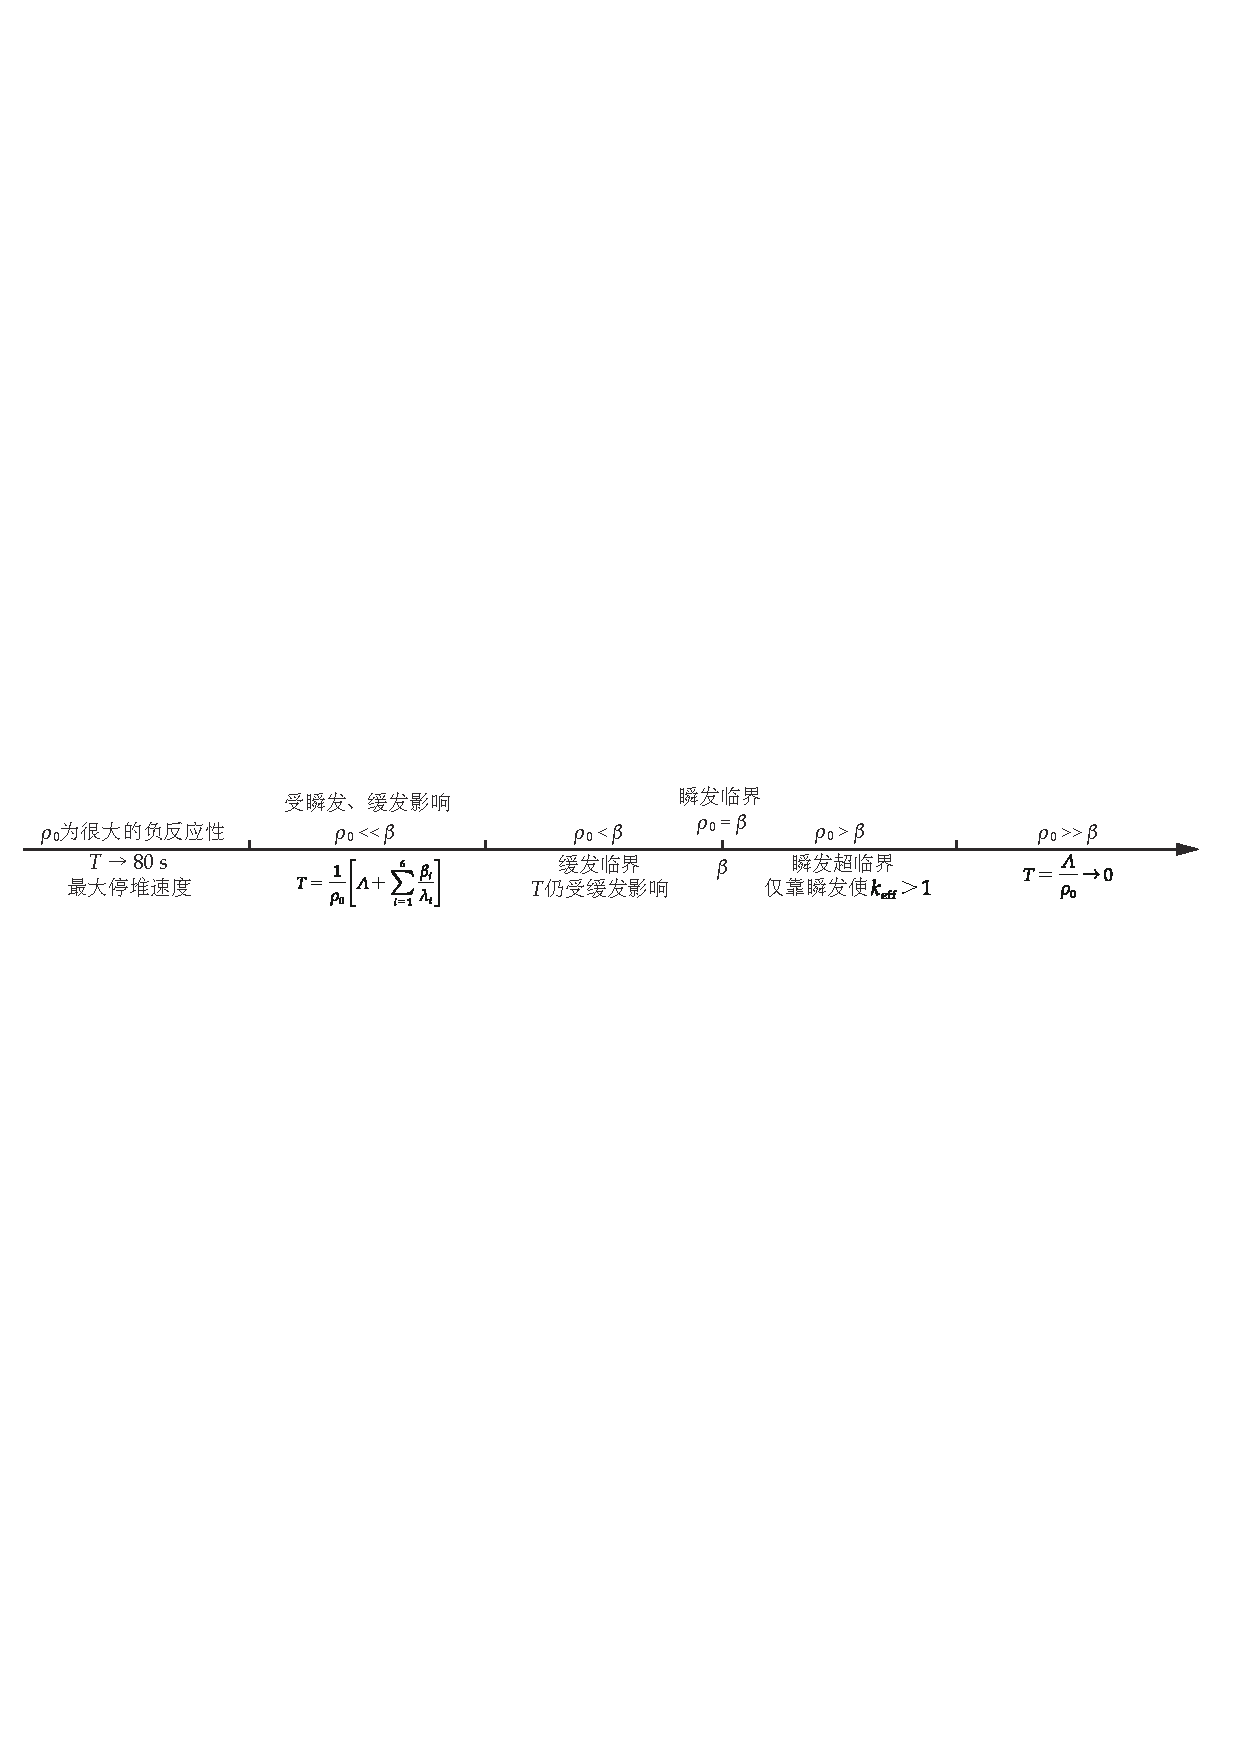
\includegraphics[scale=0.7]{figures/figure4.1.pdf}
\end{figure}

\subsection{核反应堆瞬态响应分析}

本节研究在反应性阶跃输入下,$n(t)$的变化规律。

\subsubsection{六组缓发}

\begin{enumerate}
    \item $\rho > 0$ \quad 开始时$n/n_0$突然上升,然后按缓发中子决定的周期增加;
    \item $\rho < \beta$ \quad 瞬发和缓发中子共同作用才会临界,$n/n0$缓慢上升,时间特性主要由缓发决定;
    \item $\rho < 0$ \quad 开始时$n/n_0$迅速下降,然后按缓发中子决定的速度下降。
\end{enumerate}

\subsubsection{等效单组}

求解过程相当繁琐,建议直接背过方程以应对考试。
\begin{align}
    &n(t) = \frac{n_0}{\beta - \rho_0} \left[\beta {\rm e}^{\frac{\lambda \rho_0}{\beta - \rho_0}t} - \rho_0 {\rm e}^{-\frac{\beta - \rho_0}{\varLambda}t}\right](\text{小阶跃}) \label{little step} \\
    &n(t) = \frac{n_0}{\rho_0 - \beta} \left[\rho_0 {\rm e}^{\frac{\rho_0 - \beta}{\varLambda}t} - \beta {\rm e}^{-\frac{\lambda \rho_0}{\rho_0 - \beta}t}\right](\text{大阶跃}) \label{big step}
\end{align}

常源近似和瞬跳近似了解即可。

\subsection{核反应堆的传递函数}

\begin{definition}[系统的传递函数]
    零初始条件下,线性定常系统输出变量拉普拉斯变换与输入变量拉普拉斯变换之比,表征系统的固有特征。
\end{definition}

\subsubsection{六组缓发}
将\cref{linear equation}做拉普拉斯变换,得
\begin{equation}
    \begin{cases}\displaystyle
        s\Delta N(s) = \frac{n_0}{\varLambda}\Delta \rho(s) + \frac{\rho_0 - \beta}{\varLambda}\Delta N(s) + \sum_{i=1}^{6} \lambda_i \Delta C_i(s) \\
        s\Delta C_i(s) = \frac{\beta_i}{\varLambda} \Delta N(s) - \lambda_i \Delta C_i(s)
    \end{cases}
\end{equation}

解得传递函数为
\begin{equation}
    K_{\rm R} G_{\rm R}(s) = \frac{\Delta N(s)}{\Delta \rho(s)} = \frac{n_0}{\displaystyle s\left(\varLambda + \sum_{i=1}^{6} \frac{\beta_i}{s+\lambda_i}\right) - \rho_0}
\end{equation}

临界时,$\rho_0 = 0$。

\subsubsection{等效单组}
同理对等效单组缓发中子线性化方程进行拉普拉斯变换,解得
\begin{equation}
    K_{\rm R} G_{\rm R}(s) = \frac{\Delta N(s)}{\Delta \rho(s)} = \frac{n_0}{\varLambda s + \frac{\beta s}{s+\lambda} - \rho_0}
\end{equation}

临界时,有
\begin{equation}
    K_{\rm R} G_{\rm R}(s) = \frac{n_0}{\varLambda} \frac{s+\lambda}{s(s+\beta/\varLambda)}
\end{equation}

离散化后,有
\begin{equation}
    K_{\rm R} G_{\rm R}(z) = \frac{n_0 T}{\varLambda} \frac{(z-1)+\lambda T}{(z-1)[(z-1)+\lambda T+\beta T/\varLambda]}
\end{equation}

常源近似和瞬跳近似也是了解即可。

\subsubsection{引入温度反馈}

燃料温度变化引起反应性效应是瞬发的,慢化剂温度变化引起的反应性效应是缓发的。

不必熟练掌握,对照课本推导,知道在题目存在温度反馈时如何使用相关物理量解题即可。

\subsection{核反应堆的频率特性}

\subsubsection{高频段}
$\varomega$增大,幅值减小,相位角$\varphi(\varomega) \to -\pi/2$,当$\varomega$足够大时,$\lambda_i$不再起作用,频率特性与缓发中子无关。

\subsubsection{低频段}
$\varomega$减小,幅值增大,相位角$\varphi(\varomega) \to -\pi/2$。

要能结合结论看懂教材图4-17。

\subsubsection{具有温度反馈}

\begin{enumerate}
    \item 低频段,$K_{\rm RT}G_{\rm RT}(j\varomega) = 1/K_{\rm TC}$,与反应堆无关,只与反馈特性有关;
    \item 高频段,$K_{\rm RT}G_{\rm RT}(j\varomega) = K_{\rm R}G_{\rm R}(j\varomega)$,与反馈特性无关,只与反应堆有关。
\end{enumerate}

\subsection{核反应堆的状态空间表达式}

\subsubsection{等效单组}
由\cref{equal linear}改写,得
\begin{align}
    \begin{bmatrix}
        \Delta \dot{n} \\
        \Delta \dot{c}
    \end{bmatrix} &= \begin{bmatrix}
        -\frac{\beta}{\varLambda} & \lambda \\
        \frac{\beta}{\varLambda} & -\lambda
    \end{bmatrix} \begin{bmatrix}
        \Delta n \\
        \Delta c
    \end{bmatrix} + \begin{bmatrix}
        \frac{n_0}{\varLambda} \\
        0
    \end{bmatrix} \Delta \rho \\
    y &= \begin{bmatrix}
        1 & 0
    \end{bmatrix} \begin{bmatrix}
        \Delta n \\
        \Delta c
    \end{bmatrix}
\end{align}

其与传递函数的关系见\cref{G}。

\subsubsection{反应性阶跃}

由\cref{equal one}改写,得
\begin{equation}
    \begin{bmatrix}
        \dot{n} \\
        \dot{c}
    \end{bmatrix} = \begin{bmatrix}
        \frac{\rho_0 - \beta}{\varLambda} & \lambda \\
        \frac{\beta}{\varLambda} & -\lambda
    \end{bmatrix} \begin{bmatrix}
        n \\
        c
    \end{bmatrix}
\end{equation}

它的近似解正是小阶跃下核反应堆的瞬态响应结果,即\cref{little step}。
\subsection{习题选解}

\begin{exercise} % 4.1
    闭环传递函数标准型为
    \begin{equation*}
        G(s) = \frac{\varomega_n^2}{s^2 + 2\xi \varomega_n s + \varomega_n^2}
    \end{equation*}
    \begin{align*}
        &G_0(s) = \frac{\frac{16}{s+0.8}}{1+\frac{16k}{s+0.8}} = \frac{16}{s+0.8+16k} \\
        &G(s) = \frac{G_0(s)\frac{1}{s}}{1+G_0(s)\frac{1}{s}} = \frac{16}{s^2 + (16k+0.8)s + 16} = \frac{4^2}{s^2 + 2\times 4 \times \frac{16k+0.8}{8}s + 4^2}
    \end{align*}
    由题意,得
    \begin{equation*}
        \xi = \frac{16k+0.8}{8} = 0.5 \Rightarrow k = 0.2
    \end{equation*}
\end{exercise}

\setcounter{exercise}{2}

\begin{exercise} % 4.3
    \begin{equation*}
        G(s) = \frac{U_o(s)}{U_i(s)} = \frac{\frac{1}{sC_2}+R_2}{\frac{1}{sC_1}\Vert R_1 + \frac{1}{sC_2} + R_2} = \frac{(1+sC_1 R_1)(1+sC_2 R_2)}{1+s(C_1 R_1 + C_2 R_2)+s^2 C_1R_1 C_2R_2}
    \end{equation*}
\end{exercise}

\setcounter{exercise}{5}

\begin{exercise} % 4.6
    这里只给出$\rho = 0.001$的情况。
    \begin{enumerate}
        \item 用增量状态空间表达式
        \begin{align*}
            \begin{bmatrix}
                \Delta \dot{n} \\
                \Delta \dot{c}
            \end{bmatrix} &= \begin{bmatrix}
                -\frac{\beta}{\varLambda} & \lambda \\
                \frac{\beta}{\varLambda} & -\lambda
            \end{bmatrix} \begin{bmatrix}
                \Delta n \\
                \Delta c
            \end{bmatrix} + \begin{bmatrix}
                \frac{n_0}{\varLambda} \\
                0
            \end{bmatrix} \Delta \rho \\
            y &= \begin{bmatrix}
                1 & 0
            \end{bmatrix} \begin{bmatrix}
                \Delta n \\
                \Delta c
            \end{bmatrix}
        \end{align*}
        这里输入为$\Delta \rho = 0.001$,代入相关量,得
        \begin{align*}
            \begin{bmatrix}
                \Delta \dot{n} \\
                \Delta \dot{c}
            \end{bmatrix} &= \begin{bmatrix}
                -70 & 0.08 \\
                70 & -0.08
            \end{bmatrix} \begin{bmatrix}
                \Delta n \\
                \Delta c
            \end{bmatrix} + \begin{bmatrix}
                10^4 n_0 \\
                0
            \end{bmatrix} \times 0.001 \\
            (s\symbfit{I} - \symbfit{A})^{-1} &= \frac{\begin{bmatrix}
                s+0.08 & 0.08 \\
                70 & s+70
            \end{bmatrix}}{s(s+70.08)}
        \end{align*}
        \begin{align*}
            {\rm e}^{\symbfit{A}t} &= \mathcal{L}^{-1}\left[(s\symbfit{I} - \symbfit{A})^{-1}\right] = \begin{bmatrix}
                \frac{1}{876}+\frac{875}{876}{\rm e}^{-70.08t} & 0.08+{\rm e}^{-70.08t} \\
                70+{\rm e}^{-70.08t} & \frac{875}{876}+\frac{1}{876}{\rm e}^{-70.08t}
            \end{bmatrix} \\
            \Delta n(t) &= {\rm e}^{\symbfit{A}t} \Delta n(0) + \int_{0}^{t} {\rm e}^{\symbfit{A}(t-\tau)} \begin{bmatrix}
                10n_0 \\
                0
            \end{bmatrix} \times 0.001 {\rm d}\tau \\
            &= 0 + \int_{0}^{t} 10n_0\left[\frac{1}{876}+\frac{875}{876}{\rm e}^{-70.08(t-\tau)}\right] {\rm d}\tau
        \end{align*}
        \item 用动态状态空间表达式
        \begin{equation*}
            \begin{bmatrix}
                \dot{n} \\
                \dot{c}
            \end{bmatrix} = \begin{bmatrix}
                \frac{\rho_0 - \beta}{\varLambda} & \lambda \\
                \frac{\beta}{\varLambda} & -\lambda
            \end{bmatrix} \begin{bmatrix}
                n \\
                c
            \end{bmatrix}
        \end{equation*}
        这里为阶跃$\rho_0 = 0.001$,代入相关量,得
        \begin{equation*}
            \begin{bmatrix}
                \dot{n} \\
                \dot{c}
            \end{bmatrix} = \begin{bmatrix}
                -60 & 0.08 \\
                70 & -0.08
            \end{bmatrix} \begin{bmatrix}
                n \\
                c
            \end{bmatrix}
        \end{equation*}
        参照教材推导流程,解得
        \begin{align*}
            n(t) &= \frac{n_0}{\beta - \rho_0} \left[\beta {\rm e}^{\frac{\lambda \rho_0}{\beta - \rho_0}t} - \rho_0 {\rm e}^{-\frac{\beta - \rho_0}{\varLambda}t}\right] \\
            &= 166.67 n_0 (0.007{\rm e}^{0.01333t}-0.001{\rm e}^{-60t})
        \end{align*}
    \end{enumerate}
    需要说明,这两种方法得到的结果并不相等,因为在推导中取的近似本就不同,相对而言,由动态状态空间表达式得到的解更为准确。
\end{exercise}
